% Created by tikzDevice version 0.12 on 2019-03-22 15:23:13
% !TEX encoding = UTF-8 Unicode
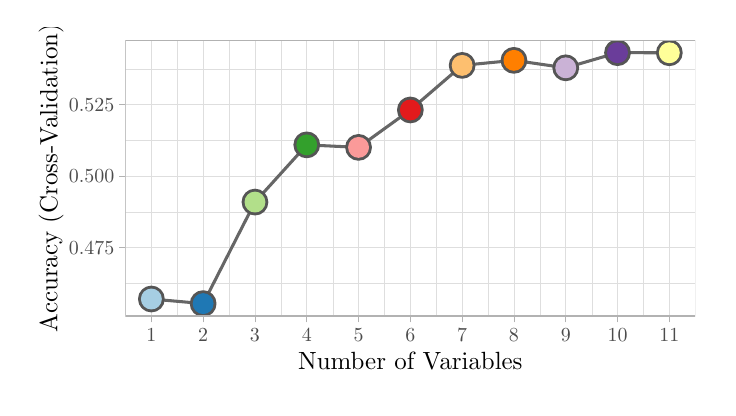
\begin{tikzpicture}[x=1pt,y=1pt]
\definecolor{fillColor}{RGB}{255,255,255}
\path[use as bounding box,fill=fillColor,fill opacity=0.00] (0,0) rectangle (245.72,130.09);
\begin{scope}
\path[clip] (  0.00,  0.00) rectangle (245.72,130.09);
\definecolor{drawColor}{RGB}{255,255,255}
\definecolor{fillColor}{RGB}{255,255,255}

\path[draw=drawColor,line width= 0.5pt,line join=round,line cap=round,fill=fillColor] (  0.00,  0.00) rectangle (245.72,130.09);
\end{scope}
\begin{scope}
\path[clip] ( 35.34, 25.85) rectangle (241.22,125.59);
\definecolor{fillColor}{RGB}{255,255,255}

\path[fill=fillColor] ( 35.34, 25.85) rectangle (241.22,125.59);
\definecolor{drawColor}{gray}{0.87}

\path[draw=drawColor,line width= 0.1pt,line join=round] ( 35.34, 37.82) --
	(241.22, 37.82);

\path[draw=drawColor,line width= 0.1pt,line join=round] ( 35.34, 63.58) --
	(241.22, 63.58);

\path[draw=drawColor,line width= 0.1pt,line join=round] ( 35.34, 89.35) --
	(241.22, 89.35);

\path[draw=drawColor,line width= 0.1pt,line join=round] ( 35.34,115.11) --
	(241.22,115.11);

\path[draw=drawColor,line width= 0.1pt,line join=round] ( 35.34, 25.85) --
	( 35.34,125.59);

\path[draw=drawColor,line width= 0.1pt,line join=round] ( 54.05, 25.85) --
	( 54.05,125.59);

\path[draw=drawColor,line width= 0.1pt,line join=round] ( 72.77, 25.85) --
	( 72.77,125.59);

\path[draw=drawColor,line width= 0.1pt,line join=round] ( 91.49, 25.85) --
	( 91.49,125.59);

\path[draw=drawColor,line width= 0.1pt,line join=round] (110.20, 25.85) --
	(110.20,125.59);

\path[draw=drawColor,line width= 0.1pt,line join=round] (128.92, 25.85) --
	(128.92,125.59);

\path[draw=drawColor,line width= 0.1pt,line join=round] (147.64, 25.85) --
	(147.64,125.59);

\path[draw=drawColor,line width= 0.1pt,line join=round] (166.35, 25.85) --
	(166.35,125.59);

\path[draw=drawColor,line width= 0.1pt,line join=round] (185.07, 25.85) --
	(185.07,125.59);

\path[draw=drawColor,line width= 0.1pt,line join=round] (203.79, 25.85) --
	(203.79,125.59);

\path[draw=drawColor,line width= 0.1pt,line join=round] (222.50, 25.85) --
	(222.50,125.59);

\path[draw=drawColor,line width= 0.1pt,line join=round] (241.22, 25.85) --
	(241.22,125.59);

\path[draw=drawColor,line width= 0.2pt,line join=round] ( 35.34, 50.70) --
	(241.22, 50.70);

\path[draw=drawColor,line width= 0.2pt,line join=round] ( 35.34, 76.46) --
	(241.22, 76.46);

\path[draw=drawColor,line width= 0.2pt,line join=round] ( 35.34,102.23) --
	(241.22,102.23);

\path[draw=drawColor,line width= 0.2pt,line join=round] ( 44.70, 25.85) --
	( 44.70,125.59);

\path[draw=drawColor,line width= 0.2pt,line join=round] ( 63.41, 25.85) --
	( 63.41,125.59);

\path[draw=drawColor,line width= 0.2pt,line join=round] ( 82.13, 25.85) --
	( 82.13,125.59);

\path[draw=drawColor,line width= 0.2pt,line join=round] (100.85, 25.85) --
	(100.85,125.59);

\path[draw=drawColor,line width= 0.2pt,line join=round] (119.56, 25.85) --
	(119.56,125.59);

\path[draw=drawColor,line width= 0.2pt,line join=round] (138.28, 25.85) --
	(138.28,125.59);

\path[draw=drawColor,line width= 0.2pt,line join=round] (156.99, 25.85) --
	(156.99,125.59);

\path[draw=drawColor,line width= 0.2pt,line join=round] (175.71, 25.85) --
	(175.71,125.59);

\path[draw=drawColor,line width= 0.2pt,line join=round] (194.43, 25.85) --
	(194.43,125.59);

\path[draw=drawColor,line width= 0.2pt,line join=round] (213.14, 25.85) --
	(213.14,125.59);

\path[draw=drawColor,line width= 0.2pt,line join=round] (231.86, 25.85) --
	(231.86,125.59);
\definecolor{drawColor}{RGB}{0,0,0}

\path[draw=drawColor,line width= 0.6pt,line join=round] ( 44.70, 32.04) --
	( 63.41, 30.38) --
	( 82.13, 67.07) --
	(100.85, 87.74) --
	(119.56, 86.83) --
	(138.28,100.35) --
	(156.99,116.46) --
	(175.71,118.28) --
	(194.43,115.58) --
	(213.14,121.05) --
	(231.86,121.02);
\definecolor{fillColor}{RGB}{0,0,0}

\path[draw=drawColor,line width= 0.4pt,line join=round,line cap=round,fill=fillColor] ( 44.70, 32.04) circle (  1.96);

\path[draw=drawColor,line width= 0.4pt,line join=round,line cap=round,fill=fillColor] ( 63.41, 30.38) circle (  1.96);

\path[draw=drawColor,line width= 0.4pt,line join=round,line cap=round,fill=fillColor] ( 82.13, 67.07) circle (  1.96);

\path[draw=drawColor,line width= 0.4pt,line join=round,line cap=round,fill=fillColor] (100.85, 87.74) circle (  1.96);

\path[draw=drawColor,line width= 0.4pt,line join=round,line cap=round,fill=fillColor] (119.56, 86.83) circle (  1.96);

\path[draw=drawColor,line width= 0.4pt,line join=round,line cap=round,fill=fillColor] (138.28,100.35) circle (  1.96);

\path[draw=drawColor,line width= 0.4pt,line join=round,line cap=round,fill=fillColor] (156.99,116.46) circle (  1.96);

\path[draw=drawColor,line width= 0.4pt,line join=round,line cap=round,fill=fillColor] (175.71,118.28) circle (  1.96);

\path[draw=drawColor,line width= 0.4pt,line join=round,line cap=round,fill=fillColor] (194.43,115.58) circle (  1.96);

\path[draw=drawColor,line width= 0.4pt,line join=round,line cap=round,fill=fillColor] (231.86,121.02) circle (  1.96);
\definecolor{drawColor}{RGB}{0,0,255}
\definecolor{fillColor}{RGB}{0,0,255}

\path[draw=drawColor,line width= 0.4pt,line join=round,line cap=round,fill=fillColor] (213.14,121.05) circle (  3.57);
\definecolor{drawColor}{gray}{0.40}

\path[draw=drawColor,line width= 1.1pt,line join=round] ( 44.70, 32.04) --
	( 63.41, 30.38) --
	( 82.13, 67.07) --
	(100.85, 87.74) --
	(119.56, 86.83) --
	(138.28,100.35) --
	(156.99,116.46) --
	(175.71,118.28) --
	(194.43,115.58) --
	(213.14,121.05) --
	(231.86,121.02);
\definecolor{drawColor}{RGB}{85,85,85}
\definecolor{fillColor}{RGB}{85,85,85}

\path[draw=drawColor,line width= 1.1pt,line join=round,line cap=round,fill=fillColor] ( 44.70, 32.04) circle (  4.28);

\path[draw=drawColor,line width= 1.1pt,line join=round,line cap=round,fill=fillColor] ( 63.41, 30.38) circle (  4.28);

\path[draw=drawColor,line width= 1.1pt,line join=round,line cap=round,fill=fillColor] ( 82.13, 67.07) circle (  4.28);

\path[draw=drawColor,line width= 1.1pt,line join=round,line cap=round,fill=fillColor] (100.85, 87.74) circle (  4.28);

\path[draw=drawColor,line width= 1.1pt,line join=round,line cap=round,fill=fillColor] (119.56, 86.83) circle (  4.28);

\path[draw=drawColor,line width= 1.1pt,line join=round,line cap=round,fill=fillColor] (138.28,100.35) circle (  4.28);

\path[draw=drawColor,line width= 1.1pt,line join=round,line cap=round,fill=fillColor] (156.99,116.46) circle (  4.28);

\path[draw=drawColor,line width= 1.1pt,line join=round,line cap=round,fill=fillColor] (175.71,118.28) circle (  4.28);

\path[draw=drawColor,line width= 1.1pt,line join=round,line cap=round,fill=fillColor] (194.43,115.58) circle (  4.28);

\path[draw=drawColor,line width= 1.1pt,line join=round,line cap=round,fill=fillColor] (213.14,121.05) circle (  4.28);

\path[draw=drawColor,line width= 1.1pt,line join=round,line cap=round,fill=fillColor] (231.86,121.02) circle (  4.28);
\definecolor{drawColor}{RGB}{166,206,227}
\definecolor{fillColor}{RGB}{166,206,227}

\path[draw=drawColor,line width= 0.4pt,line join=round,line cap=round,fill=fillColor] ( 44.70, 32.04) circle (  3.57);
\definecolor{drawColor}{RGB}{31,120,180}
\definecolor{fillColor}{RGB}{31,120,180}

\path[draw=drawColor,line width= 0.4pt,line join=round,line cap=round,fill=fillColor] ( 63.41, 30.38) circle (  3.57);
\definecolor{drawColor}{RGB}{178,223,138}
\definecolor{fillColor}{RGB}{178,223,138}

\path[draw=drawColor,line width= 0.4pt,line join=round,line cap=round,fill=fillColor] ( 82.13, 67.07) circle (  3.57);
\definecolor{drawColor}{RGB}{51,160,44}
\definecolor{fillColor}{RGB}{51,160,44}

\path[draw=drawColor,line width= 0.4pt,line join=round,line cap=round,fill=fillColor] (100.85, 87.74) circle (  3.57);
\definecolor{drawColor}{RGB}{251,154,153}
\definecolor{fillColor}{RGB}{251,154,153}

\path[draw=drawColor,line width= 0.4pt,line join=round,line cap=round,fill=fillColor] (119.56, 86.83) circle (  3.57);
\definecolor{drawColor}{RGB}{227,26,28}
\definecolor{fillColor}{RGB}{227,26,28}

\path[draw=drawColor,line width= 0.4pt,line join=round,line cap=round,fill=fillColor] (138.28,100.35) circle (  3.57);
\definecolor{drawColor}{RGB}{253,191,111}
\definecolor{fillColor}{RGB}{253,191,111}

\path[draw=drawColor,line width= 0.4pt,line join=round,line cap=round,fill=fillColor] (156.99,116.46) circle (  3.57);
\definecolor{drawColor}{RGB}{255,127,0}
\definecolor{fillColor}{RGB}{255,127,0}

\path[draw=drawColor,line width= 0.4pt,line join=round,line cap=round,fill=fillColor] (175.71,118.28) circle (  3.57);
\definecolor{drawColor}{RGB}{202,178,214}
\definecolor{fillColor}{RGB}{202,178,214}

\path[draw=drawColor,line width= 0.4pt,line join=round,line cap=round,fill=fillColor] (194.43,115.58) circle (  3.57);
\definecolor{drawColor}{RGB}{106,61,154}
\definecolor{fillColor}{RGB}{106,61,154}

\path[draw=drawColor,line width= 0.4pt,line join=round,line cap=round,fill=fillColor] (213.14,121.05) circle (  3.57);
\definecolor{drawColor}{RGB}{255,255,153}
\definecolor{fillColor}{RGB}{255,255,153}

\path[draw=drawColor,line width= 0.4pt,line join=round,line cap=round,fill=fillColor] (231.86,121.02) circle (  3.57);
\definecolor{drawColor}{gray}{0.70}

\path[draw=drawColor,line width= 0.5pt,line join=round,line cap=round] ( 35.34, 25.85) rectangle (241.22,125.59);
\end{scope}
\begin{scope}
\path[clip] (  0.00,  0.00) rectangle (245.72,130.09);
\definecolor{drawColor}{gray}{0.30}

\node[text=drawColor,anchor=base east,inner sep=0pt, outer sep=0pt, scale=  0.72] at ( 31.29, 48.22) {0.475};

\node[text=drawColor,anchor=base east,inner sep=0pt, outer sep=0pt, scale=  0.72] at ( 31.29, 73.98) {0.500};

\node[text=drawColor,anchor=base east,inner sep=0pt, outer sep=0pt, scale=  0.72] at ( 31.29, 99.75) {0.525};
\end{scope}
\begin{scope}
\path[clip] (  0.00,  0.00) rectangle (245.72,130.09);
\definecolor{drawColor}{gray}{0.70}

\path[draw=drawColor,line width= 0.2pt,line join=round] ( 33.09, 50.70) --
	( 35.34, 50.70);

\path[draw=drawColor,line width= 0.2pt,line join=round] ( 33.09, 76.46) --
	( 35.34, 76.46);

\path[draw=drawColor,line width= 0.2pt,line join=round] ( 33.09,102.23) --
	( 35.34,102.23);
\end{scope}
\begin{scope}
\path[clip] (  0.00,  0.00) rectangle (245.72,130.09);
\definecolor{drawColor}{gray}{0.70}

\path[draw=drawColor,line width= 0.2pt,line join=round] ( 44.70, 23.60) --
	( 44.70, 25.85);

\path[draw=drawColor,line width= 0.2pt,line join=round] ( 63.41, 23.60) --
	( 63.41, 25.85);

\path[draw=drawColor,line width= 0.2pt,line join=round] ( 82.13, 23.60) --
	( 82.13, 25.85);

\path[draw=drawColor,line width= 0.2pt,line join=round] (100.85, 23.60) --
	(100.85, 25.85);

\path[draw=drawColor,line width= 0.2pt,line join=round] (119.56, 23.60) --
	(119.56, 25.85);

\path[draw=drawColor,line width= 0.2pt,line join=round] (138.28, 23.60) --
	(138.28, 25.85);

\path[draw=drawColor,line width= 0.2pt,line join=round] (156.99, 23.60) --
	(156.99, 25.85);

\path[draw=drawColor,line width= 0.2pt,line join=round] (175.71, 23.60) --
	(175.71, 25.85);

\path[draw=drawColor,line width= 0.2pt,line join=round] (194.43, 23.60) --
	(194.43, 25.85);

\path[draw=drawColor,line width= 0.2pt,line join=round] (213.14, 23.60) --
	(213.14, 25.85);

\path[draw=drawColor,line width= 0.2pt,line join=round] (231.86, 23.60) --
	(231.86, 25.85);
\end{scope}
\begin{scope}
\path[clip] (  0.00,  0.00) rectangle (245.72,130.09);
\definecolor{drawColor}{gray}{0.30}

\node[text=drawColor,anchor=base,inner sep=0pt, outer sep=0pt, scale=  0.72] at ( 44.70, 16.84) {1};

\node[text=drawColor,anchor=base,inner sep=0pt, outer sep=0pt, scale=  0.72] at ( 63.41, 16.84) {2};

\node[text=drawColor,anchor=base,inner sep=0pt, outer sep=0pt, scale=  0.72] at ( 82.13, 16.84) {3};

\node[text=drawColor,anchor=base,inner sep=0pt, outer sep=0pt, scale=  0.72] at (100.85, 16.84) {4};

\node[text=drawColor,anchor=base,inner sep=0pt, outer sep=0pt, scale=  0.72] at (119.56, 16.84) {5};

\node[text=drawColor,anchor=base,inner sep=0pt, outer sep=0pt, scale=  0.72] at (138.28, 16.84) {6};

\node[text=drawColor,anchor=base,inner sep=0pt, outer sep=0pt, scale=  0.72] at (156.99, 16.84) {7};

\node[text=drawColor,anchor=base,inner sep=0pt, outer sep=0pt, scale=  0.72] at (175.71, 16.84) {8};

\node[text=drawColor,anchor=base,inner sep=0pt, outer sep=0pt, scale=  0.72] at (194.43, 16.84) {9};

\node[text=drawColor,anchor=base,inner sep=0pt, outer sep=0pt, scale=  0.72] at (213.14, 16.84) {10};

\node[text=drawColor,anchor=base,inner sep=0pt, outer sep=0pt, scale=  0.72] at (231.86, 16.84) {11};
\end{scope}
\begin{scope}
\path[clip] (  0.00,  0.00) rectangle (245.72,130.09);
\definecolor{drawColor}{RGB}{0,0,0}

\node[text=drawColor,anchor=base,inner sep=0pt, outer sep=0pt, scale=  0.90] at (138.28,  6.44) {Number of Variables};
\end{scope}
\begin{scope}
\path[clip] (  0.00,  0.00) rectangle (245.72,130.09);
\definecolor{drawColor}{RGB}{0,0,0}

\node[text=drawColor,rotate= 90.00,anchor=base,inner sep=0pt, outer sep=0pt, scale=  0.90] at ( 10.70, 75.72) {Accuracy (Cross-Validation)};
\end{scope}
\end{tikzpicture}
